\documentclass{usydthesis}

% Configuration

\def\degree{Bachelor of Information Technology (Honours)}
\def\department{School of Information Technologies}

\title{{\bf\Huge Large Scale Multi-output and Probabilistic Benthic Habitat Mapping}}
\author{Justin Ting}
\def\sid{430203826}
\def\supervisor{Dr. Simon O'Callaghan}
%\def\assocsupervisor{Comment this line to remove assoc supervisor}

%%%%%%%%%%%%
% Packages

\usepackage{alltt}
\usepackage[export]{adjustbox}
\usepackage{amsfonts}
\usepackage{amsmath}
\usepackage{amsthm}
\usepackage{amsthm}
\usepackage{animate}
\usepackage[toc,page]{appendix}
\usepackage[english]{babel}
\usepackage{caption}
\usepackage{hyperref}
\usepackage[all]{hypcap}
\usepackage{graphicx}
\usepackage{listings}
\usepackage{longtable}
\usepackage{media9}
\usepackage{multirow}
\usepackage{pdflscape}
\usepackage{pgf}
\usepackage{pifont}
\usepackage{qtree}
\usepackage[english,rounding]{rccol}
\usepackage{rotating}
\usepackage[section]{placeins}
% \usepackage[subsection]{placeins}
\usepackage{setspace}
\usepackage{style/bib}
% \usepackage{subfigure}
\usepackage[caption=false]{subfig}
\usepackage{tabularx}
\usepackage{tipa}
\usepackage{wrapfig}
\usepackage{xcolor}
\usepackage{xspace}
\usepackage{cleveref}

% Column width macros
\usepackage{array}
\newcolumntype{L}[1]{>{\raggedright\let\newline\\\arraybackslash\hspace{0pt}}m{#1}}
\newcolumntype{C}[1]{>{\centering\let\newline\\\arraybackslash\hspace{0pt}}m{#1}}
\newcolumntype{R}[1]{>{\raggedleft\let\newline\\\arraybackslash\hspace{0pt}}m{#1}}

\theoremstyle{definition}
\newtheorem{ex}{Example}[section]

\graphicspath{{images/}}
\addmediapath{images/}

\rcDecimalSignOutput{.} % rccol

\newenvironment{sidewaystablepage}{\begin{landscape}\begin{table}}{\end{table}\end{landscape}}

\def\subsectionautorefname{Section}
\def\subtableautorefname{Table}
\def\subfigureautorefname{Figure}
\def\chapterautorefname{Chapter}

\newcommand{\tick}{\ding{51}}
\newcommand{\cross}{\ding{53}}

\newcommand{\todo}[1]{{\color{red} #1}}
\newcommand{\sent}[1]{{\color{blue}\texttt{#1}\xspace}}

\DeclareMathOperator{\logit}{logit}
\DeclareMathOperator{\logistic}{logistic}
\DeclareMathOperator{\Dir}{Dir}
\DeclareMathOperator{\dirmul}{DirMult}
\DeclareMathOperator{\B}{B}
\DeclareMathOperator{\softmax}{softmax}

%%%%%%%%%%%%
% Maths functions
\def\O{\mbox{O}}

%%%%%%%%%%%%
% Setup

%   Page size:
\oddsidemargin=0cm	% really 1in
\evensidemargin=0cm
\textwidth=6.2677165in

% initial page numbers:  i, ii, iii, ...
\renewcommand{\thepage}{\roman{page}}

\newcommand{\defn}[1]{\textit{#1}}
\newcommand{\ttl}[1]{\textit{#1}}
\newcommand{\txt}[1]{\textsf{\smaller #1}}
\newcommand{\qu}[1]{\textsf{#1}}
\newcommand{\txtbf}[1]{\textsf{\textbf{\small #1}}}
\newcommand{\quot}[1]{\textit{#1}}

\newcommand{\sssection}[1]{\textsf{\textbf{#1}}}

\newcommand{\cf}[1]{\mbox{$\it{#1}$}}   % category font

\newcommand{\alta}{\textsc{alta}\xspace}
\newcommand{\api}{\textsc{api}\xspace}
\newcommand{\candc}{C\&C\xspace}
\newcommand{\ccg}{\textsc{ccg}\xspace}
\newcommand{\ccgbank}{CCGbank\xspace}
\newcommand{\cky}{\textsc{cky}\xspace}
\newcommand{\jhu}{\textsc{jhu}\xspace}
\newcommand{\lfg}{\textsc{lfg}\xspace}
\newcommand{\hpsg}{\textsc{hpsg}\xspace}
\newcommand{\mwe}{\textsc{mwe}\xspace}
\newcommand{\mwes}{\mwe{}s\xspace}
\newcommand{\NE}{\textsc{ne}\xspace}
\newcommand{\Naive}{Na\"{i}ve\xspace}
\newcommand{\naive}{na\"{i}ve\xspace}
\newcommand{\ngram}{$n$-gram\xspace}
\newcommand{\ngrams}{\ngram{}s\xspace}
\newcommand{\nlp}{\textsc{nlp}\xspace}
\newcommand{\np}{\textsc{np}\xspace}
\newcommand{\nps}{\np{}s\xspace}
\newcommand{\parseval}{\textsc{parseval}\xspace}
\newcommand{\pos}{\textsc{pos}\xspace}
\newcommand{\pp}{\textsc{pp}\xspace}
\newcommand{\qa}{\textsc{qa}\xspace}
\newcommand{\ram}{\textsc{ram}\xspace}
\newcommand{\rasp}{\textsc{rasp}\xspace}
\newcommand{\tbl}{\textsc{tbl}\xspace}
\newcommand{\ptb}{\textsc{ptb}\xspace}
\newcommand{\wsj}{\textsc{wsj}\xspace}

\newtheorem*{definition}{Definition}
\newtheorem*{assumption}{Assumption}
\newtheorem*{mainassumption}{Main Assumption}
\newtheorem*{corollary*}{Corollary}




%%%%%%%%%%%%
% Start

\begin{document}

%%%%%%%%%%%%
% Title page
\maketitle

\setstretch{1.5}

% intro pages
\cleardoublepage
\phantomsection
\chapter*{Student Plagiarism: Compliance Statement} \label{sec:plagiarism}
{
\setlength{\parindent}{0cm}
\setlength{\parskip}{1em}

I certify that:   

I have read and understood the University of Sydney Student Plagiarism:  Coursework Policy and Procedure;

I understand that failure to comply with the Student Plagiarism: Coursework Policy and Procedure can lead to the University commencing proceedings against  me for potential student misconduct under Chapter 8 of the University of Sydney  By-Law 1999 (as amended);  

This Work is substantially my own, and to the extent that any part of this Work  is not my own I have indicated that it is not my own by Acknowledging  the Source of that part or those parts of the Work.  
}

\vspace{4cm}
\begin{tabular}{llll}
\textbf{Name}: & \authors & &  \\[2em]
\textbf{Signature}: & \hspace{0.4\textwidth} & \textbf{Date}: & \hspace{0.4\textwidth}\\[2cm]
\end{tabular}




\cleardoublepage
\phantomsection
\chapter*{Abstract}

Being able to predict the state of benthic habitats based on limited information is crucial for environmental conservation, particularly as the impact of human activity on our oceans is greater than ever before. A considerable portion of work done in the area uses deterministic methods that strictly assign only one label to a given bathymetry data point, while more advanced models provide probabilistic results over all possible labels at any one point, also similarly only representing a single output. However, like the majority of real life classification problems \todo{(citation here perhaps)}, habitat mapping is intrinsically a multi-label problem for any data collected at a resolution low enough to be economically feasible to be performed at a large scale. In this paper, we explore advantages of having probabilistic class outputs as well as treating benthic habitat mapping as a multi-output problem particularly when faced with relatively low resolution bathymetry data, compared to the primary method of deterministic, single-output methods explored in existing literature.

\cleardoublepage
\phantomsection
\chapter*{Acknowledgements}

The thanks go in here.



% tables
\cleardoublepage
\setcounter{tocdepth}{2}
\setcounter{secnumdepth}{4}
\tableofcontents

{\makeatletter
\renewcommand*\numberline[1]{\hb@xt@\@tempdima{#1 \hfil}\hspace*{1em}}
\makeatother
% \listoffigures
% \listoftables
\cleardoublepage
}

%%%%%%%%%%%%
% Chapters
\setcounter{page}{1}
\setcounter{chapter}{0}

% main page numbers:  1, 2, 3, ...
\renewcommand{\thepage}{\arabic{page}}	
\setupParagraphs

\todo{maybe put a notation section?}
\chapter{Introduction}

Earth's oceans cover 70\% of its surface, but only less than 10\% of the Earth's oceans have been explored to date\footnote{Oceanservice.noaa.gov. (2016). How much of the ocean have we explored?. [online] Available at: http://oceanservice.noaa.gov/facts/exploration.html}. There have been increasing efforts over the past few decades to more efficiently map out these unexplored areas to monitor marine ecosystems to be able to track the state of them over time for reasons such as management and preseveration purposes. The process used is called benthic\footnote{Benthic refers to things relating to the bottom of the ocean, i.e. the ocean floor} habitat mapping and involves generating predictive maps of different habitat types at the ocean floor. Most efforts to create benthic habitat maps share some basic key steps - acoustic data is used to estimate properties about the surface of the benthos, then its relationship with other `truthing' data such as images or video are inferred. 

Early attempts at this understanding and modeling these relationships would have been expert-driven where any map created by an individual or individuals would be fully subject to their personal biases and knowledge. With the lack of better tools available, this was the best option - until machine learning algorithms began to be formulated more formally, and applied to real world problems. Thus, deterministic methods such as random forests and support vector machines made their debut, and enabled predictions on large sets of potentially complex data that would have previously proved to be a considerable challenge or even impossible when done manually, and would have required major compromises. 

However, considering that the creation of habitat maps would be for conservation of marine management purposes, it would be important to be able to state the confidence of the predictions are made, a property that deterministic methods do not possess. Gaussian processes are a complex model that can provide this information - providing both the probability of every label being the `correct' one at a certain data point, as well as the variance on each of these predictions. Due to the $O(n^3)$ matrix inversion steps involved in them, the time that would be required to fit a Gaussian process to more beyond several thousand points would be astronomical and impractical for any real world applications. To account for this, there exist approximations such as product of experts and Bayesian committee machines that allow levels of parallelism of the model (that are inapplicable to the basic Gaussian process) that are (almost) bounded only by hardware. 

These methods so far ignore the fact that asynchronously collected bathymetry and image data will often not correspond to one another in a $1:1$ manner (as is the case in this study), with each bathymetry point likely related to several images. This results in a dataset where for each coordinate with bathymetry data, the labels across several labels are attributed to it, or in other words, a vector of label counts. As the aforementioned models do not handle such data, approximations were made where these vectors were simplified down to a single label, throwing out a majority of the information that was collected. To actually fully utiliese these vector counts, a method is needed that can model this data appropriately - such as the Dirichlet Multinomial. This allows predictions to be made over category counts, providing normalised predictions at each point, not only correctly interpreting the data in contrast to other methods used in benthic habitat mapping, but also allowing properties of the benthos such as biodiversity and co-habitation to be directly inferred from the data, not requiring additional post-processing steps.

% It is the relationship which is inferred between the different data sets inferred using machine learning techniques that varies between studies. A considerable portion of such studies are shown to use deterministic methods to predict a label for any given coordinate such as Random Forests and Support Vector machines (SVMs), whilst more recent ones make use of more informative methods such as Gaussian Processes, providing a distribution over all possible labels given any data point.

\section{Contribution}

The main contributions of this thesis are twofold. Fistly, an investigation into current probabilistic methods is performed. Gaussian proceses are a state-of-the-art method in this regard, although the implementations of them available in open source libraries and the like are currently unable to work with datasets larger than several thousand points without hitting computational limits, which makes them impractical for real-world use, if, for example, trying to fit a model for data prediction alone for several tens of thousands of points could take weeks, if not longer. This work seeks to investigate whether recent innovations in the field are able to improve performance sufficiently that it can be used on larger datasets, and in particular, to the specific field of benthic habitat mapping.

The second aim is to explore the use and modelling of information where input data does not only have a single label such as `sand', but could have a category count over labels, such as $7$ counts of sand, $3$ counts of coral, and $1$ count of rhodliths, also representible as a normalised distribution $[0.7, 0.3, 0.1]$. Such data is collected as a result of automated underwater vehicles (AUV) collecting  images at the ocean floor at a density of, for example, one every $10m^2$, whereas bathymetry data is collected from the ocean surface at a lower rate, such as $50m^2$. This means there can be more than one image, and hence habitat label per bathymetry data point, where any single image is `assigned' to the nearest bathymetry data point. While this can be used with single-output machine learning algorithms, it involves simplifying every data point's label distribution to only the most dominant label - in the aforementioned example, $[0.7, 0.3, 0.1]$ would be simplified to sand. Although this allows common and readily available methods to be used, it also discards a considerable amount of otherwise useful information. To fully utilise all this information, use of the Dirichlet Multinomial distribution to model the data is explored, along the other information that can be gathered from it such as measurements of biodiversity and entropy to represent confidence in predictions.
% \todo{(need to rewrite most of this. investigating probabilistic methods and improving their performance as well)} The main contribution of this thesis will be to explore how to use data where a single data point does not have only one label exclusively, but instead corresponds to a tally of each possible label. For example, a particular 5m x 5m area in the benthos may be an even mix of both sand and coral, but in previous literature, the data was simplified such that whichever label occurred more frequently regardless of how small the margin would be the single label assigned to that point. This results in a very coarse approximation even when using Gaussian Processes attempts to model the uncertainty/uncertainty with its predictions at each point (but ultimately only provides a single, final prediction). To alleviate this and provide a richer set of information, we explore the use of Dirichlet Multinomials, which provides a distribution of each label that represents something entirely different. Whereas in a Gaussian Process, each label is assigned the probability of being the correct one, the output of a Dirichlet Multinomial Regressor provides the distribution of the frequency of labels in a particular space itself. See section \todo{GP vs DM} for an illustrative example on how results would differ in practice between the two methods.

\section{Motivation}
The motivation for exploring the aforementioned technical aspects of benthic habitat mapping is to explore how the process of benthic habitat mapping can be performed more economically while also providing richer information than has generally been the case in such efforts, and also automating as much of the process as possible. To break down the three aims mentioned - the economic aspect comes into play in terms of density at which the data is collected. Naturally, collecting more data would cost more money - being able to work with coarser data where multiple images may correspond to single bathymetry data point using a technically sound method that can make full use of the data has the potential to cut down on the need to collect huge amounts of data. Richer information can be obtained both from the probabilistic component of Gaussian processes as well as the Dirichlet distribution's entropy from the Dirichlet multinomial. This is necessary because any actions taken to manage or conserve benthic habitats inherently comes with a level of risk whether it be environmental or economical, and quantifying this risk would require that at the very least, the mathematical models used to form predictions need to be able to state their confidence.

% \todo{(motivation for speeding up GP?)} The motivation behind assessing the effectiveness and advantages of such a method are that they inherently tie in with lower resolution data, particularly when a single bathymetry points corresponds to a large enough area such that one would expect a mix of different labels. This is advantageous because we want to be able to re-sample data from any given site periodically (for example, every 3-4 years) whilst being economically efficient. This naturally lends to lower resolution data, meaning that summarising large areas to a single label would theoretically be throwing away a majority of the information contained in bathymetry and image data.

\section{Outline}

We will first review some of the existing literature in \Cref{chap:relatedworks}, on the collection of bathymetry and image data briefly, then on deterministic approaches to benthic habitat mapping to date, such as logistic regression, and random forests, and their performance on varying types of benthic environments. This is in contrast to the more informative probabilistic and multi-output approaches that will be explained in \Cref{chap:gps} and \Cref{chap:dms}, where we look at the mathematical background behind Gaussian processes and Dirichlet multinomial regression. In \Cref{chap:experiments}, we then apply the techniques explained in the previous chapters and observe their performance, points of interest, as well as how the information obtained differs to methods visited in explored in the related works. This is followed by \Cref{chap:evaluation}, an evaluation of the experiment designs, as well as the limitations that were present and how they could have affected the study. The study is then concluded and summarised in \Cref{chap:conclusion}, discussing the possible impact of this work, as well as areas of the study that could be explored in further detail as possible future work.

\chapter{Literature Review} \label{chap:litreview}

%%%%%%%%%%%%%%%%%%%%%%%%%%%%%%%%%%%%%%%%%%%% OVERVIEW %%%%%%%%%%%%%%%%%%%%%%%%%%%%%%%%%%%%%%%%%%%%
In this chapter, we will first provide an overview of what benthic habitat mapping is and the general steps involved in data collection and how it is used, followed by a review of some of most commonly used approaches when performing benghic habitat mapping. The notion of benthic habitat mapping precedes the rapid developments in machine learning methods in recent history, and as such, early attempts would naturally have involved manual predictions based on available information that would be subject to the biases of experts involved in the process. It is then natural to expect that given the same raw data, different experts who have had varying experiences in their field would come to different conclusions. This was observed in a geoscience related study \citep{bond07}, where 

           \section{Overview}
            The process of benthic habitat mapping involves three key steps that the large majority of all studies in the area go through.\footnote{Ozcoasts.gov.au. (2016). Benthic habitat mapping: Mapping Overview. [online] Available at: http://www.ozcoasts.gov.au/geom\_geol/toolkit/mapoverview.jsp}. In this section, we will give a brief overview of each of these steps, along with common procedures used in them across studies in this area.

            \begin{enumerate}
                \item \textbf{Habitat Characterisation} - extracting properties of the environment such as rugosity (roughness), aspect (direction of slope), depth
                \item \textbf{Habitat Classification} - grouping the raw information about the environment into categories, such as sand, granite, etc.
                \item \textbf{Habitat Mapping} - using classifications with the larger scale bathymetry data to extrapolate habitat maps 
            \end{enumerate}

            %%%%%%%%%%%%%%% Habitat Characterisation %%%%%%%%%%%%%%%
            \subsection{Habitat Characterisation}
            \todo {not just resolution of data but modality. images vs bathymetry} If we were able to collect high resolution data for the entire ocean's benthos - the job of creating benthic habitats for any given area would be (relatively) trivial. As this is prohibitively expensive, we instead collect large amounts of low resolution data, and small samples of high resolution data (between which we model a relationship). This subsection provides a brief summary of data collected and methods used to do so.


            \paragraph{Remote-sensing data}
            Due to the cost of sea expeditions, it is economically infeasible to have marine vehicles (autonomous or otherwise) explore the entire ocean floor to confirm the ecological properties of all of Earth's benthos. However, we do need to collect sufficiently detailed data of large areas at a time, partiulcarly those of being mapped, and for this, remote-sensing data is used. These usually come in the form of acoustic backscatter data that involes the firing of sound waves towards the benthos, whereby their frequency and strength upon returning is used to deduce the depth of a particular material, as well the density of said material (from which a guess at the actual substance can be made - e.g. sand, mud, etc.).

            Multibeam echosounders (MBES) are becoming a more frequently used method of collecting acoustic backscatter data ~\citep*{calvert15} despite older methods involving single beam echo sounders (SBES) being cheaper and easier to segment. This stems from the fact that the reduced cost comes at the expense of (potentially) accuracy, as well as lower resolution data. This is due to SBES' beam angle, i.e. the angle formed by the 2D flattening of the 'cone' shape of the emitted beams, ranging from 15-25$^{\circ}$, whereas MBES' is 0.5-3$^{\circ}$, depending on the particular system~\citep*{cjbrown11}. The difference in angle means that data returned via SBES devices are more 'coarse', reprsenting less accuracy and granularity, whereas that of MBES is more detailed and can present more information. However, there is overhead associated with use of MBES, in that the considerably decreased angles means much more 'overalpping' data, adding complexity to the segmentation process.

            \paragraph{Truthing Data}
            \todo{explain redundancy here, unclear what it's referring to - why is there redundancy?} The most common methods to be able to obtain a sufficiently large truthing data set (but still trivially small compared to the area covered by remote-sensing data) are videos or images - though the former still requires post-processing to extract the needed images. The advantage that can be provided here, however, is the redundancy in data points ~\citep*{rattray14}  - but there is extra cost in time required to convert videos into the needed images (pre-proessing before feeding into algorithms for habitat mapping), an area that is in itself worth of research within the field.~\citep*{lucieer13}

            \paragraph{Other data}
            \todo{(why is water column correction important when correlating images with seagrass standing crop?)} Other data that is less common, but also used to map habitats, is patterns in the water movement (such as tidal currents, wave action)~\citep*{cjbrown11} in the column of water above the area of benthos being mapped - a feature that provided useful input in arriving at an accurate benthic habitat map (in addition to sediment analysis).~\citep*{snelgrove94} Other sources such as UNESCO have also verified the importance and significance of using water column correction techniques to obtain more accurate habitat maps, particularly when correlating images with segrass standing crop. \footnote{Unesco.org. (2016). Water column correction techniques. [online] Available at: http://www.unesco.org/csi/pub/source/rs10.htm} 

            %%%%%%%%%%%%%%% Habitat Classification %%%%%%%%%%%%%%%
            \section{Habitat Classification}

            \todo{more in-depth focus here, what kind of supervised/unsupervised ML algorithms are used for classification?} Almost all studies use \textit{in situ} 'truthing' data to complement the acoustic data to be able to build a model between the acoustic data and truthing data (creation of these models are explained in following sections). However, we need to know the labels of this data considering that the final goal is to create a habitat map, where any one habitual zone is given its prospetive label - to do this, we also need to label the clusters of truthing data. These categories may be, for example, 'bedrock covered by discontinuous seagrass cover', 'Maerl interspersed with sand and gravel', 'superficially coarse sand to fine gravel covered by dense patches of seagrass', etc.~\citep{micallef12}. The two overarching ways to perform this classification are in the form of supervised and unsupervised algorithms.


            Studies have used both supervised and unsupervised methods in clustering the initial data for the training step. Often, there may be large amounts of visual data, beyond that which any human or even team can reasonably, manually cluster - and as such, unsupervised algorithms are first used to create these clusters, after which an expert may be brought in to verify/simplify (or otherwise) the resulting clusters.~\citep*{steinberg11} 

            \section{Map Creation}
            The final step is map creation, which many papers related to benthic habitat mapping focus on - and also where the most variation occurs in terms of the method used. The various approaches used can be categorised into two broad categories. The first is a top down approach whereby the classification of the habitat characterisation data is validated (or otherwise) with the truthing data, and the second is a bottom up approach where the characterisation data is similarly clustered into classes, but not to directly represent a particular habitat - instead, the aim is to find a relationship between the acoustic data clusters and the truthing data clusters which we can model. Using this model, we can then extrapolate the acoustic data which doesn't have corresponding truthing data to create the habitat map.~\citep{ahsan11} We will explore this aspect more when looking at how the mapping process has evolved over time and the improvements that it has brought about.

            %%%%%%%%%%%%%%% Non-ML Habitat Mapping %%%%%%%%%%%%%%%
            \section{Non-Machine Learning Approaches} 
            \todo{this section should be part of the previous one (Map Creation)} While the majority of modern papers in benthic habitat mapping employ machine learning techniques for map creation, this doesn't exclude those that do not from providing useful information and insight. An important study was undertaken in 2001 that employs relatively basic statistical analysis, employing different forms of variance as its main tool of analysis. ~\citep{kostylev01}, at the time (and in fact, even now) integrated more sources of data together than most other studies undertaken - multibeam bathymetric data, geoscientific data, seafloor photographs, habitat complexity, and relative current strength. Rather than drawing broad conclusions about the effectiveness of a collection of tools in creating habiatat maps, deeper analysis is done on subsets of the data to attempt to clarify some of the complexities and intrinsic properties of benthic habitats and ecosystems themselves. Although little is done to address and verify accuracy of the actual results/map in this paper, it provides value through the analysis of variance and covariance performed on and between different benthic/marine properties, establishing relationships typically taken for granted or ignored. For example, it is established that while sediment type contirubted heavily to a higher taxonomic group count, there was little relationship between sediment type and depth. However, this only indicates that there is no linear relationship between the two, and doesn't necessarily preclude a non-linear relationship between them, perhaps with the inclusion of other parameters as well. In particular, Kostylev establishes that gravel subrates are more abundant with varying taxonomic groups than their sand counterparts.

            Certain organisations, government bodies/etc. will also provide guidelines outlining the classification proess. For example, the European Nature Information System website and the Australian Government's 'Interim Marine and Coastal Regionalisation for Australia'\footnote{Unesco.org. (2016). Water column correction techniques. [online] Available at: http://www.unesco.org/csi/pub/source/rs10.htm} both provide classification schemes for people creating habitat maps or other similar efforts.

            Such findings provide useful insights for future studies that will allow a better assessment of data, or to be able to apply initial assumptions in obtaining better results. However, constantly seeking a deeper understanding through a proportionally increasing amount of sampling creeps towards 'exploring' the entire Earth's oceans manually. To obtain economically feasible yet reliable predictions from the limited data that we have, we need to employ machine learning techniques to fully utilise the information that we gather.

            %%%%%%%%%%%%%%%%%%%%%%%%%%%%%%%%%%%%%%%%%%%%% Evolution of Map Creation Methods %%%%%%%%%%%%%%%%%%%%%%%%%%%%%%%%%%%%%%%%%%%%%
            \section{Machine Learning in Benthic Habitat Mapping}
            As benthic habitat mapping covers a diverse range of discplines, namely "marine biology, ecology, geology, hydrography, oceanography and geophysics"~\citep{cjbrown11}, in addition to statistics and machine learning, it is logical that it would take considerable effort and vast resources to give each relevant discpline an equal, and large amount of attention within any single study. Thus, different papers can rely on collective findings of others to launch their own research and look further into particular lines of inquiry, start new ones altogether, or evaluate effectiveness of methods used in the field/etc. Within benthic habitat mapping, one prevalent line of inquiry is how to create more accurate, higher quality maps by employing machine learning techniques. For the remainder of this review, we will be revisiting common machine learning techniques and their application in the various stages of benthic habitat mapping along with the benefits they provide.

            \subsection{Deterministic Machine Learning Algorithms}
            In this section, we will review some machine algorithms that can be used in benthic habitat mapping processes - whether that be in the initial clustering stages of (ideally) independently gathered datasets such as acoustic backscatter data and collections of high resolution images, or the actual classification of 'new' (or testing) data in determining their predicted habitat classes.

            \paragraph{Multinomial Logistic Regression}
            Multiple Logistical Regression is one of the more basic machine learning algorithms that can be used to predict habitat classes, and falls under the 'supervised learning' category as we have the 'output' for the feature vector in the intial data. Regression, broadly, involves the estimation of relationships between variables, and logistic regression involves the prediction of likelihood of class membership given a number of variables (that are assumed to have low collinearity). This only applies to domains with two classes, however - to use this technique for classification where we have an unbounded (though usually still relatively low) number of classes, we need to use multinomial logistic regression, which is able to account for more than two distinct, unordered (i.e., sand vs. mud has no relative ordering) classes, where class membership is predicted using maximum likelihood estimation (MLE), similarly to logistic regression. However, the difference is that whereas logistic regression only requiring a single logit function as its nominal variable is dichotomous, multinomial logistic regression requires comparison between $k-1$ (where $k$ is the number of possible dependent variables) logit functions. 

            Even though ~\citet{caruana06} show that logistic regression methods achieve on average worse results than most other approaches available, it recognises that in certain cases the models that perform most poorly on average still display exceptional performance, and as such, this method is still worth exploration and experimentation. In particular, ~\citet{belanger12} used multinomial logistic regression across temperature, salinity, and productivity to correctly predict class membership by a margin of 23-84\% more than by pure chance. This is equivalent to an improvement of 1-2x compared to a random guess, which taken at face value would suggest that logistic regression is an undesirable choice of algorithm for this problem domain.

            \paragraph{Random Forests}
            In contrast to logistic regression, random forests were shown in ~\citet{caruana06} to be state of the art, only just falling short of boosted decision trees after callibration. Random forests are an ensemble method, meaning that it uses a collection of estimators, before aggregating their results to obtain some sort of average. The aim of this is to minimise the variance and hence error that any single one of these estimators would otherwise result in. 

            From the initial dataset, some number $B$ is chosen which represents the \textit{number} of trees to build (as a part of our random forest), after which, $B$ random, unique subsamples of the full dataset are taken. Within each decision tree in our random forest, some constant number $m$ of features is taken at each node of the tree, such that the split at each node only takes into account the $m$ randomly chosen features. Each of the decision trees in our forest will hence have a 'result' (that may be a class or some continuous value). Typically, the final decision of the random forest will be made by a vote count for classification, and an average of each decision tree's result in regression problems.

            As random forests are a method that is low in complexity but provides very good results on average, we can see that it is used in quite a few studies (~\citet{lucieer13}, ~\citet{seiler12}, ~\citet{hasan14}), where the random forest classifier provided the best results over other methods relating to at least a significant subset of the explored data. However, ~\citet{lucieer13} found that while random forest classifiers were most able to classify substratum and rugosity, K-nearest neighbour classifiers most accurately classified sponge structure classes, pointing to the need to do a more systematic comparison of different methods in benthic habitat mapping. A further advantage to using random forests as pointed out in ~\citep{hasan14} is that it can provide insight into which features were more important than others, which can aid future studies to be more successful and efficient by focusing more efforts towards collecting the most influential data. The success met with using random forests make it a good benchmark to compare against for future work that aim to develop methods to create more accurate benthic habitat maps than has been done before.

            \paragraph{Multi-class Support Vector Machines}
            Although support vector machines fell outside the top three overall supervised learning algorithms in terms of performance (accuracy), their non-parametricity could potentially be of benefit given that our knowledge of the complex relationships between elements of benthic habitats are limited. Moreover, despite SVMs being rarely used anywhere in the field, they are "acknowledged to be very competitive descriminative classifiers in machine learning literature"~\citep{ahsan11}.

            However, SVMs in their base form only support classification into two classes, requiring modification to the original algorithm to support more - an active area of research that has not found any single 'best' way to perform this algorithm extension yet. To do so, there are two, basic main approaches available, one being a \textbf{one vs. all} approach, and the other being a combination of all \textbf{one vs. one} approach. We can hence quite clearly see that given $C$ possible classes, the first would require $C$ separate classifiers, whereas the latter would require $\frac{C(C-1)}{2}$ classifiers~\citep{murphy12}. Multi-class SVMs were used in ~\citet{ahsan11} for illustrative purposes, using the one vs. one approach as per their use of LibSVM~\citep{chang11}, outperforming classification trees on certain datasets, and in limited cases (but not overall), Gaussian Mixture Models as well. Again, the mixed results would suggest that under certain conditions (such as size of the dataset and various properties of the data itself, some of which are not known before testing), use of a multi-class SVM could provide a useful benchmark to some extent.

            %%%%%%%%%%%%%%% Probabilistic Methods %%%%%%%%%%%%%%%
            \subsection{Probabilistic Methods}
            The classifications being made regarding benthic habitats naturally involve uncertainty, as we are still learning the relationship between differnt characteristics of benthos with the varying communities of fauna and flora that reside there. Whilst guessing the most likely class for a particular domain deterministically has its practical applications, it is arguably more \textit{natural} to represent the uncertainty ~\citep{rasmussen06}. As our understanding of marine environments is still quite weak ~\citep{un04}, it is debatable whether deterministic results are always appropriate when being used to make high level management decisions relating to marine environments. While deterministic methods will create a model that attempts to explicitly account for all variables, probabilistic models deal with joint distributions over all the variables. As we need to better understand "the complexities of coastal system functioning rather than simplfying and scaling down the system into smaller components" ~\citep{diaz04}, this feature can be esepcially valuable seeing as there is simply not enough 'expert knowledge' to adequately, explicitly model the relationship across a range of variables.

            \paragraph{Illustrative Example} \todo{not an illustrative example - give some actual figures/graph of crossover point} A simple example of this can be seen when comparing the deterministic approach of a logistic regression classifier, with the probabilistic Naive Bayes classifier. Starting from no data, up until a certain threshold, a Naive Bayes (NB) classifier will actually provide a more accurate classification as it approaches its comparatively higher asymptoptic quicker, after which point, one there is sufficient data, the logistic regressor will provide the better results ~\citep{ng04}. In this simplified example, an analogy can be drawn where the data used up to the threshold when the NB classifier performs better represents a lack of knowledge about the data causing the logistic regressor to underperform, where as the continued addition of data represents more understanding (more data points) of the domain, allowing logistic regression to then outperform the NB classifier.

            \paragraph{Gaussian Mixture Models} Gaussian mixture models (GMMs) are parametric models that "model the distribution of data as a set of clusters, where each cluster is a multivariate Gaussian"~\cite{ahsan11}. In this particlar paper, GMMs are compared with classification trees, which it is found to perform better than in most cases, but were also predicted classes from unseen data with higher certainty than discriminative methods. This is because of its generative nature that accounts for the distribution of bathymetric features, allowing it to model the joint distribution of the classes as well as features. Moreover, each \todo{(function = distribution)}Gaussian function within the model has its own mean and covariance matrix, which also contributes to its powerful modeling ability. However, the use of GMM may have been hindered by the dimensionality of the data - while only five properties were measured, each was calculated for a varying number of scales for the input vector, meaning the 'features' were at least some multiple of five. As this exceeds the recommended six dimensions for use with GMM, application to a very large dataset may be beyond reasonable computational ability.\footnote{Nickgillian.com. (2016). GMM Classifier — NickGillianWiki. [online] Available at: http://www.nickgillian.com/wiki/pmwiki.php/GRT/GMMClassifier}. To avoid this, the feature vector may have to be truncated to contain the bathymetric properties for only one particular scale at a time.

            \paragraph{Using Gaussian Processes} A recent study used probabilistic methods to develop a mapping between the clustered acoustic data to continuous cluster probabilities, as opposed to discrete cluster labels, thus representing the certainty of the results obtained. Using Gaussian Processes which do not inherently support classification, ~\citet{bender12} extended the probabilistic least squares classifier to retain the information regarding certainty of class membership that exists during the classfication process, rather than discarding it in the traditional method. By evaluating the probabilistic results of PTLSC by comparing its results with the actual cluster probabilities obtained in the classification of the images via an unsupervised variational Dirichlet process model, it was shown that the PTLSC method performed better than a PLSC trained directly on the discrete cluster labels in terms of accuracy, mean squared error, and mean variance as well. This demonstrates that while both PTLSC and PLSC err in their predictions when dealing with the transition different boundaries, by maintaining probabilistic information in the PTLSC, it is able to make slightly better judgements in such cases.

            \paragraph{Gaussian Processes and large datasets} However, Gaussian processes involve a matrix inversion process that requires an O($n^3$) operation which does not scale well with large datasets. To overcome this whilst reaping the benefits of Gaussian processes, ~\citet{bender12} extracted subsets of the original dataset on which to perform analysis - a small, randomly chosen portion from three Gaussians, of the initial millions of observations. While this has still provided a high accuracy for all methods tested, there is likely information to be gained by being able to use a considerably larger portion of the dataset. To do this, a method would be required to generate sparse covariance matrices through approximations ~\citep{bickel08}, or use of functions that guarantee sparseness as a property~\citep*{melkumyan09} - something that can be explored in future work. To illustrate how the obstacle can be overcome, the latter paper describes a method whereby, rather than inverting the covariance matrix in its raw form, a threshold is calculated at which point, rather than observing the normal 'tapering' off of covariance values, they are simply set to zero beyond that point. This will result in a significant portion of the covariance matrix being populated with 0s, at which point inversion of the sparse matrix can be performed for which there are known efficient methods. However, there have been more ways of sparse approximation GPs that other studies have explored.

            \paragraph{Sparse Approximation Gaussian Processes}

            \todo{m isn't clarified here, plus n<m is incorrect, should be m<<n} 

            \todo{lots of things here have become irrelevant (talks about 'optimal' methods that aren't implemented/included in experiments - limit to relevant ones, i.e. the GP ensemble methods}

            It is of importance that a number of methods of dealing with sparse approximation of GPs are taken into account if the aim is to deal with large GPs in the inversion step. ~\citep{candela05} explores exactly this, immediately discounting the "subset of data" (SoD) method as being non-competitive due to it not being able to represent the original data to a reasonably accurate enough extent, though we have seen that this was the approach taken in ~\citep{bender12}. As all the different methods (bar SoD) have a complexity of $O(nm^{2})$ where $n$ is the size of the data, and $n<m$, the authors notably point out that no gross approximations should be made as more competent methods are computationally equivalent, and as such point towards their notes on future work to outperform the existing state of the art. As such, we would wish to explore combining the \textbf{Partially Independent Training Conditional approximation} with "the most powerful selection method for the inducing inputs." 


\chapter{Probabilistic Classification for Large Datasets}\label{chap:gps}

The methods of habitat mapping explored until now were mostly deterministic ones, where predictions were absolute, and as such did not provide a \textit{level of confidence} in the predictions made, or in other words, probabilistic output. When using information provided by predictive benthic maps, decisions being made will often have far-reaching impacts, and as such all parties involved need to be as well informed as possible. Machine learning techniques such as SVMs cannot provide probabilistic outputs, so despite being popular in machine learning literature, is not the best fit for modeling ocean habitats if intended for real world use. Gaussian processes are state of the art in terms of probabilistic modeling, and a method that has seen some attention in the area of benthic habitat mapping, though it is still considerably less common than more traditional methods like SVMs and random forests.

In this section, we will look at Gaussian processes as a technique to generate predictive habitat maps. We begin by going over the basics of Gaussian process regression, and how a small extension/post-processing step extends it to allow Gaussian process classification. Due to the covariance matrix inversions needed during the training stage, Gaussian processes have an $O(n^3)$ complexity, severely restricting the number of points we can work with. Approximation methods are explored as a way to overcome this constraint, and their performance as well as runtime required to fit models and predict data is compared to a normal Gaussian process. Detailed proofs and derivations are not covered in this chapter, and interested readers should consult Rasmussen and William's Gaussian Processes for Machine Learning book ~\citep{rasmussen06} for a definitive guide to all things Gaussian process related. In particular, Chapters 2 and 5 are of the most relevance, as they detail Gaussian process regression, and model selection and adaptation of hyperparameters respectively.

% $\mathbf{f_*}$ - predictive function outputs corresponding to input data $X_*$
 \section{Gaussian Process Regression}\label{chapsec:gpr}

Compared to deterministic methods like linear regression\footnote{Strictly speaking, linear regression is a Gaussian process with a linear kernel - but due to its simplicity, and that Gaussian processes are not usually explained by weight coefficients but by their hyperparmeters, we are juxtaposing linear regression to Gaussian processes here as a simpler approach.} that explains data by optimising $\mathbf{y=X\beta} + \epsilon$, where $\mathbf{y}$ are the response variables, $\mathbf{X}$ are the input variables, and $\mathbf{\beta}$ are the regression coefficients, Gaussian process regression takes a Bayesian approach by adjusting probabilities when given more information (input data), and performs inference over functions.

We define a Gaussian process on input $\mathbf{x}$ to have a mean function $m$ and covariance function $k$ (or in other words, the kernel), where $\mathbf{x}$ and $\mathbf{x'}$ are the training and test inputs respectively:
\begin{equation}
f(x) \sim GP(m(\mathbf{x}), k(\mathbf{x}, \mathbf{x'}))
\end{equation}

The chosen kernel is the squared exponential, represented by the covariance function between points $p, q$, where $\mathbf{x_p, x_q}$ are the vector of features at each point is thus given by:
\begin{equation}\label{eq:simplegpcov}
    cov(f(\mathbf{x_p}), f(\mathbf{x_q)}) = k(\mathbf{x_p, x_q}) = \exp(-\frac{1}{2}|\mathbf{x_p}-\mathbf{x_q}|^2)
\end{equation}

The free parameters involved in the squared exponential kernel are the length scales $l$, signal variance $\sigma_f$ and noise variance $\sigma_n$, and need to be optimised to perform predictions on unseen data.
\begin{equation}\label{eq:fullgpcov}
    k\mathbf{(x_p, x_q)} = \sigma^2_f \exp(-\frac{1}{2l^2} (\mathbf{x_p-x_q})^2) + \sigma^2_nI
\end{equation}
where $\sigma_f$ is the variance in the training data, and $\sigma_n$ is the variance of the Gaussian noise. The length scales $l$ are not a single variable as the equation may suggest, but a vector of length scales equal in length to the number of dimensions in the inputs $\mathbf{x}$. If $l$ was simply a vector of 1s, which would give every feature in the input space equal weighting, but it is not likely in a real world dataset for every feature to have equal importance. This is what the length scales account for - by tuning $l_i$ for each feature $i$, the model can learn during the fitting process which features are important, and which ones are not. 

 The equations for the predictive means and variances then incorporate the covariance function, and hence the hyperparameters, as follows:
\begin{equation}
    \bar{f_*} = \mathbf{k_*}^T(K+\sigma_n^2)^{-1} \mathbf{y}
\end{equation}
\begin{equation}
    \mathbb{V}[f_*] = k(\mathbf{x_*},\mathbf{x_*}) - \mathbf{k_*}^T (K+\sigma^2_n)^{-1}\mathbf{k_*}
\end{equation}
where $K = K(X, X)$ is the covariance matrix over all training points, and $\mathbf{k_*} = \mathbf{k(x_*}, X)$ is the covariance between a single test point with all training points.

% To allow simplifications of notation in the following equations, we define some abbreviations related to \autoref{eq:fullgpcov} depending on what data is involved in the covariance matrix. 
%  
%  \todo{(lay out these abbreviations nicely)}
%  To indicate the full covariance matrix over training points: $$K = K(X, X)$$
%  To indicate the full covariance between training points and test points: $$K_* = K(X, X_*)$$
%  To indicate the covariance between a single test point with all training points: $$\mathbf{k_*} = \mathbf{k(x_*}, X)$$

Data was generated in \Cref{fig:gphp_ex} below to illustrate a Gaussian process's behaviour when different hyperparameters (as shown below each plot) are used to perform regression. The key things to observe in these 2D examples are that the noise and length scale govern the complexity of the model - both a low length length scale and error are required to create a Gaussian process that attempts to adhere to points as closely as possible, though this can result in `overfitting' of the data, seems to be the case in plot 3.

\begin{figure}
    \centering
    \begin{minipage}{0.53\linewidth}
        \includegraphics[width=0.9\linewidth]{gp_with_variance_plot3.pdf}
        \caption*{(1) $\sigma_f = 2.13$, $l = 1.27$, $\sigma_n = 0.17$}
    \end{minipage}
    \hfill
    \begin{minipage}{0.47\linewidth}
        \includegraphics[width=0.9\linewidth]{gp_with_variance_plot1.pdf}
        \caption*{(2) $\sigma_f = 1$, $l = 1.7$, $\sigma_n = 0.1$}
    \end{minipage}
    \begin{minipage}{0.47\linewidth}
        \includegraphics[width=0.9\linewidth]{gp_with_variance_plot2.pdf}
        \caption*{(3) $\sigma_f = 1$, $l = 0.3$, $\sigma_n = 0.001$}
    \end{minipage}
    \label{fig:gptoyplots}
    \caption{Examples of a Gaussian process' behaviour with different hyperparameters.}
    \label{fig:gphp_ex}
\end{figure}


\section{Leave-One-Out Cross Validation}

To determine the hyperparameters of the training data, cross-validation for model training is used, with the number of folds used, $k$, equal to the number of datapoints, only excluding one data point per round - hence the name. By optimising over the sum of cross-valiated log likelihoods, it is no longer strictly only assessing the log marginal likelihood, instead acting as more of a pseudo-likelihood. Directly optimising over the marginal likelihood provides the probability of observed data \textit{given model assumptions}, whereas the cross-validation approach provides the log predictive probability estimates independent of the fufilment of said model assumptions. \citep{wahba90} states in Chapter 4 that Gaussian cross validation methods are more robust to misspecification, including problems such as non-Gaussian errors. Cross-validation was chosen for this reason, as the intrinsic properties of the data were not studied in detail prior to performing experiments as a part of this study, and nor were biological experts consulted for the duration of the study to provide advice on the quality and soundness of predictive maps.

The log probability of the data ommitting training case $i$ from the $n$ input data points is:

$$\log p(y_i|X, \mathbf{y_{-i}}, \theta) = -\frac{1}{2}\log\sigma^2_i - \frac{(y_i - \mu_i)^2}{2 \sigma^2_i} - \frac{1}{2}\log2\pi$$

for input data $X$, the $i-th$ response variable $y$, predictive mean $\mu$, and predictive variance $\sigma^2$. The total log probability across all $n$ subsets of the data of size $n-1$ is then:

$$ L_{LOO}(X, y, \theta) = \sum^n_{i=1} \log p(y_i, X, \mathbf{y_{-i}}, \mathbf{\theta})$$

The LOO-CV predictive mean and variance can then be derived, and represented in terms of covariance matrix $K$, as calculated using \Cref{eq:simplegpcov} and \Cref{eq:fullgpcov}.
$$\mu_i= y_i - \frac{[K^{-1}\mathbf{y}]_i}{[K^{-1}]_{ii}} \text{ and } \sigma_i^2 = \frac{1}{[K^{-1}]_{ii}}$$

To be able to optimise hyperparemeters over the feature dimensions more efficiently, the partial derivates over \textit{each} is also needed:
$$\frac{\partial{u_i}}{\partial{\theta_j}} = \frac{[Z_j \alpha]}{[K^{-1}]_{ii}} - \frac{\alpha_i[Z_j K^{-1}_{ii}]_{ii}}{[K^{-1}]^2_{ii}}$$
$$\frac{\partial{\sigma_i^2}}{\partial{\theta_j}} = \frac{[Z_jK^{-1}]_{ii}}{[K^{-1}]^2_{ii}}$$

$$ \text{where } \alpha = K^{-1}\mathbf{y} \text{ and } Z_j = K^{-1} \frac{\partial{K}}{\partial{\theta_j}} $$

With the means to perform Gaussian process regression by determining the hyperparameters of the kernel using leave-one-out cross-validation, the next step would be to apply this to Gaussian process classification.

\section{Gaussian Process Classification} \label{chapsec:gpc}

As benthic habitat mapping requires the prediction of discrete labels and not continuous values, Gaussian process regression is not directly applicable to the problem domain. Just as logistic regression can be formulated by post-processing of the results of a linear regressor, Gaussian process classification can be performed by using multiple Gaussian process regressors as its underlying model. The one-vs-all approach is taken in this case, requiring $k$ separate Gaussian process regressors.

For example in \Cref{fig:ova-example}, when fitting a regressor for the green \textit{class 1}, the labels at coordinates corresponding to label $1$ are set to $1$, and all other points to $0$. For \textit{blue} label $2$, the labels of all the blue points are set to $1$, and the rest $0$, and so on so forth - this is applicable to any number of classes $k$, where the complexity increases linearly for each class that exists in the data.

\begin{figure}
    \includegraphics[scale=0.5]{ova_example.pdf}
    \caption{Simple example of data being split up to perform one-vs-all classification. The coloured lines corresponding to the label colours indicate the separation of clusters when performing each round of one-vs-all regression rounds. For class $3$, everything below the red line is taken to be the `positive label', and everything above, the `negative label'. This is only illustrative, and the labels will just as easily be wrangled if they were interspersed instead of segregated like they are here.}
    \label{fig:ova-example}
\end{figure}

When forming predictions, each of these separate Gaussian process regressors provide a different set of results as they consider separate one-vs-all cases as previously trained. For the $k$ labels, and each regressor $GP_k$, where $i=1,2...,k$:

\begin{equation}
    \mathbf{\bar{f_*}_{all}} = \begin{bmatrix}
        \mathbf{\bar{f_*}_{GP_1}} \\
        \mathbf{\bar{f_*}_{GP_2}} \\
        \ldots \\
        \mathbf{\bar{f_*}_{GP_{k-1}}} \\
        \mathbf{\bar{f_*}_{GP_k}} \\
    \end{bmatrix}, \mathbf{\mathbb{V}[f_*]_{all}} = \begin{bmatrix}
        \mathbf{\mathbb{V}[f_*]_{GP_1}} \\
        \mathbf{\mathbb{V}[f_*]_{GP_2}} \\
        \ldots \\
        \mathbf{\mathbb{V}[f_*]_{GP_{k-1}}} \\
        \mathbf{\mathbb{V}[f_*]_{GP_k}} \\
    \end{bmatrix}
\end{equation}

As the original labels were changed to be constrained in the range $[0, 1]$, the same is done to the predictive means, by passing it through the logistic sigmoid function (\Cref{eq:logistic}). The resulting matrix of predictive means and variances for any $k > 1$ provides a vector of $k$ predictions for each input rather than the single label that classification would require. To simplify the probabilistic results per label at each point, the value with the highest probability (i.e. the argmax) would be taken, along with the matching variance containing the confidence intervals. As the $O(n^3)$ operations required for the matrix inversions for performing Gaussian process regression must be performed $k$ times in total (once per label), the time required for anything more than several thousand points would make it impractical to use, requiring methods to sufficiently bring down the running time.

% \section{Subsampling for Gaussian Process experiments}
% \todo{(may need to take this section out - GPy wrapper deals with thousands of points no problem, no longer need to subsample with only 4000 after downsampling the data)}
% 
% Due to the $O(n^3)$ complexity of training a Gaussian Process Classifier, using all $16502$ points was infeasible, so it was necessary to use only a subsample of the training data. As can be seen in the above histograms \todo{(reference the figure instead. may need to combine them into one)}, the distribution of classes in both the simplified and non-simplified versions was very uneven. As a result of this skew, randomly sampling the the training data to fit our GP classifier against resulted in worse results than samplying an equal \textit{number} of points for each class. To obtain a reasonably well-performing set of 1000 points (the number chosen to obtain a balance between performance and time required), 10-fold cross validation was performed on random subsets of this size. To obtain the 1000 datapoints, both stratified sampling, as well as obtaining ratios of labels matching those in the training set were used. After 200 runs, the set with the best performance was used for the remaining GP experiments.

\section{Gaussian Process Approximation} \label{chapsec:gp-approx}

To be able to use Gaussian processes on larger data sets, approximations can be made to avoid paying the full cost of performing expensive operations, approximations can be made. The method of approximation that will be used in this study is ensemble methods. In the context of Gaussian processes, this involves breaking up the data into small chunks, where each `expert' performs regression seperately, before taking the product of all the experts' results to give the approximation for the full dataset. The property that these ensemble methods have in common are that any given expert's decisions are weighted by their precision (inverse of variance - so a low variance would result in a high precision), such that experts that are more `confident' in their results provide great input to the final weightings, whereas experts with low precision, or predictions that have a high variance, are unsure of their results, and hence provide comparably less input to the summarised predictions. The component that differs between the two approximations below (and these ensemble methods in general) is how the precision of each expert is used to weight their predictions.

\subsection{Product of Gaussian Process Experts}
The product of experts algorithm is a the simplest of Gaussian process ensemble methods, as the predictive variance of expert is directly used as-is to weight that particular expert's predictions, as shown in the equations below. The \textit{product} of experts described above is proportional to a single Gaussian process with the following product of expert (PoE) predictive mean and variance:

\begin{equation}
    \mu_*^{poe} = (\sigma_*^{poe})^2 \sum_k \sigma_k^{-2} (\mathbf{x_*}) \mu_k (\mathbf{x_*})
\end{equation}
\begin{equation}\label{eq:poe-precision}
    (\sigma_*^{poe})^{-2} = \sum_k \sigma_k^{-2} (\mathbf{x_*})
\end{equation}
where $\sigma_k^{-2}(\mathbf{x_*})$ are the predictive Gaussian precisions (inverse of Gaussian variances), and $\mu_k(\mathbf{x_*})$ are the predictive Gaussian means. \Cref{eq:poe-precision} describes the precision of the product of experts model in its entirety, by summing up the Gaussian precisions of all of the experts. For each point, this means that its PoE variance will be low if every expert calculates a low predictive variance, whereas if a sufficient number of them end up predicting a high variance for a given point, the overall PoE variance for that point will likely be high. This high variance is then applied to the PoE predictive means at every point, where the the product of each \textit{individual} expert's Gaussian precisions and Gaussian means are taken, and summed with all the other experts' at the same point, giving a higher precision ($\sigma_k^{-2}(\mathbf{x_*})$) a higher weight.

\begin{equation}
    \mu_*^{gpoe} = (\sigma_*^{gpoe})^2 \sum_k \beta_k \sigma_k^{-2} (\mathbf{x_*}) \mu_k (\mathbf{x_*})
\end{equation}
\begin{equation}
    (\sigma_*^{gpoe})^{-2} = \sum_k \beta_k \sigma_k^{-2} (\mathbf{x_*})
\end{equation}

The only difference in generalised product of Gaussian experts (GPoE) is the use of $\mathbf{\beta}$, where its purpose is to allow the explicit weighting of experts based on the circumstances. The value of each $\beta_k$ is flexible, but as scaling Gaussian processes to large datasets isn't the primary focus of this study, we simply set each $\beta_k$ to $\frac{1}{M}$, where $M$ is the number of experts, as suggested in \citep{deisenroth15} to be able to maintain reasonable margins of error. To show how they perform, below is a performance comparison between these two ensemble methods on a simple dataset:
\begin{figure}[H]
    \begin{minipage}{0.49\linewidth}
        \includegraphics[width=\linewidth]{gp_poe_with_variance_plot.pdf}
        \caption*{Product of Experts}
    \end{minipage}
    \hfill
    \begin{minipage}{0.49\linewidth}
        \includegraphics[width=\linewidth]{gp_gpoe_with_variance_plot.pdf}
        \caption*{Generalised Product of Experts}
    \end{minipage}
    \caption{\scriptsize{Examples of Gaussian process ensemble methods. As a result of the $\beta$ in the GPoE scaling the variances, they no longer cancel each other out when summed together, explaining the comparatively larger variance in the GPoE compared to the PoE, even when predictions are very close to the correct values. While these conservative (wide) variances can be a negative aspect as mentioned in \citet{deisenroth15}, it may also prove to be beneficial, as the experiments later show.}}
\end{figure}

% \subsection{Bayesian Committee Machine}
% \begin{equation}
%     \mu_*^{bcm} = (\sigma_*^{bcm})^2 \sum_{k=1}^M \sigma_k^{-2} (\mathbf{x_*}) \mu_k (\mathbf{x_*})
% \end{equation}
% \begin{equation}
%     (\sigma_*^{bcm})^{-2} = \sum_{k=1}^M \sigma_k^{-2} (\mathbf{x_*}) + (1-M)\sigma_{**}^{-2}
% \end{equation}
% where $\sigma_{**}^{-2}$ is the prior precision of $p(f_*)$, which itself is the inverse of the prior variances.
% 
% \subsection{Robust Bayesian Committee Machine}
% \begin{equation}
%     \mu_*^{rbcm} = (\sigma_*^{rbcm})^2 \sum_k \beta_k \sigma_k^{-2} (\mathbf{x_*}) \mu_k (\mathbf{x_*})
% \end{equation}
\section{Summary}

In this section, we explored the probabilistic capabilities of Gaussian processes regression, and how this translates into Gaussian process classification. As these presented very restrictive limits on the size of data that can be worked with, methods to estimate them by breaking down the algorithm into emabarrasingly parallelisable chunks were explored, along with how they compare in terms of performance. It would amiss at this point not to address the existence of multi-output Gaussian processes that can work with vectors of outputs for a given input datapoint~\citep{alvarez09}. However, the multi-output that they deal with is over arbitrary ranges. Because in this particular domain, normalised predictions per point must sum to $1$ (or the original total label count at a point, in the case of training data), multi-output Gaussian processes do not enforce this constraint, and as such, their use was not explored in this study. Without a way to correctly model the multi-output data using Gaussian processes, other methods that are able to need to be explored.


\chapter{Dirichlet Multinomial Regression} \label{chap:dms}

Dirichlet multinomial regression, as the name suggestions, combines dirichlet and multinomial distributions to achieve the combined model. In particular, we are interested in modeling a distribution over category counts, as there exists relationship in our data such that every bathmetry point corresponds to a certain count of each possible label in the relevant area of benthos. \todo{explain why we should first revisit dirichlet, multinomial distributions separately before looking at dirichlet multinomial regression}

\section{Multinomial Distribution}
\todo {equations, description}

\section{Dirichlet Distribution}
\todo{descriptions}

$$\theta \sim Dir(\alpha) \text{ , dirichlet distributed random variable}$$ 
$$p(\theta)= \frac{1}{\beta(\alpha)} \Pi_{i=1}^n \theta_i^{\alpha_i - 1} I(\theta \in S) \text{ density function, I is indicator function}$$ 
$$ \theta = (\theta_1, ..., \theta_n), \alpha = (\alpha_1,...,\alpha_n), \alpha_i > 0 \text{ theta - n-dimensional vectors, alpha - parameters for distribution}$$
$$ S = \{x \in R^n : x_i \geq 0, \sum x_i = 1\} \text{ S is probability simplex, the set of pmfs on numbers 1 through n}$$ 
$$\frac{1}{\beta(\alpha)} = \frac{\Gamma(\alpha_0)}{\Gamma(\alpha_i) ... \Gamma(\alpha_n)}, \alpha_0 = \sum_{i=1}^n \alpha_i \text{ generalised beta function}$$

\section{Dirichlet Multinomial Regression}

\todo{descriptions}

$$DM(C|\alpha) = \frac{M!}{\Pi_k C_k!} \frac{\Gamma(\sum_k \alpha_k)}{\Gamma(\sum_k c_k + \alpha_k)} \Pi_{k=1}^k \frac{\Gamma(C_k + \alpha_k)}{\Gamma(\alpha_k)}$$
$$ M = \sum_k c_k $$

For the regressor, the two activation functions that were considered were exponential and softmax, where the former often provided better mapping predictions, but the latter is preferable in the general case due to its better numerical stability \todo {include graphs of exponential and softmax here}.
$$\alpha_k = \exp\{x^T w_k\}$$
$$\alpha_k = \text{softmax}\{x^T w_k\}$$

The weights $w$ here are in fact a matrix of weights with dimensions $(K \times D)$, where $K$ is the number of possible labels across the dataset, and $D$ is the dimensionality of the dataset. Muliplying the dirichlet multinomial prior by the likelihood then then gives the posterior over which to optimise to obtain the weights required to predict the normalised label counts at any given point.

This gives the joint-log-likelihood over both the dirichlet and multinomial distributions:
\begin{multline}
    \sum^N_{n=1} [\log(M_k) - \sum_k \log(c_k!) + \log \Gamma(\sum_k \alpha_k(x_n)) - \log \Gamma(\sum_k c_{nk} + \alpha_k(x_n))] \\
    + \sum^N_{n=1} \sum^K_{k=1} [\log \Gamma(c_k + \alpha(x)) - \log \Gamma(\alpha_k(x_n))] \\
    + \sum^K_{k=1} [-\frac{\phi}{2} \log(2\pi \phi) - \frac{1}{2}w_k^T \phi \mathbb{I} w_k]
\end{multline}

To optimise this equation, the partial derivative of the above over the weights $w$ are considered:
\begin{multline}
    \partial \frac{\log p(c, x)}{\partial w_k} = \sum_{n=1}^N x_n \alpha_k (x_n) [\psi(\sum_l \alpha_l(x_n)) - \psi(\sum_k c_{nk} + \alpha_k(x_n))] \\
    + \sum^N_{n=1} x_n \alpha_k (x_n) [\psi (c_{nk} + \alpha_k(x_n)) - \psi(\alpha_k(x_n))] - \frac{1}{\phi} w_k
\end{multline}

\todo {explain all the symbols here}

\subsection{Using MCMC instead of MAP}
\section{Illustrative Example}

The differences between a Gaussian Process that provides the probability distribution of possible labels compared to the Dirichlet Multinomial Regressor that provides the distribution of actual labels at a point, are highlighted in the illustrative example below. Note that three clusters were synthesised, with clusters A, B containing $0.7:0.3$ and $0.3:0.7$ average ratios in label mix per point respectively, while cluster C contained an even $0.5:0.5$ average split, where cluster had $100$ points. The colours on the overall plot are only representative of the \textbf{most} common label at each point - the actual distributions at each point are shown in the graphs following it.

% \todo{generate toy example with a mixed label A,B region and separate regions of mostly A, mostly B respectively}

\begin{figure}[H]
    \includegraphics[scale=0.7]{toydataplot.pdf}
    \caption{Plots of the three clusters, with labels taking on the argmax of each point}
    \label{fig:toyplot}
\end{figure}

\begin{figure}[H]
    \includegraphics[trim={0 2cm 0 2cm}]{toyplot_hist_distr_legend.pdf}
    \caption{Legend/axes for the following histogram plots showing distribution of labels at each point}
    \label{fig:toyplothist_legend}
\end{figure}

\begin{figure}[H]
    \begin{minipage}{.49\linewidth}
        \includegraphics[width=\linewidth]{toy_clusterA_distr.pdf}
        \caption{Label distribution of cluster A}
        \label{fig:toyclusterA}
    \end{minipage}
    \hfill
    \begin{minipage}{.49\linewidth}
        \includegraphics[width=\linewidth]{toy_clusterB_distr.pdf}
        \caption{Label distribution of cluster B}
        \label{fig:toyclusterB}
    \end{minipage}
    \begin{minipage}{.49\linewidth}
        \includegraphics[width=\linewidth]{toy_clusterC_distr.pdf}
        \caption{Label distribution of cluster C}
        \label{fig:toyclusterC}
    \end{minipage}
\end{figure}

In this example, the GP and DM models were each trained on half of each cluster, and made to predict the other half. However, as a standard GPC can only have single label inputs and outputs, a approximation/simplification was made for the purpose of calculating average error, whereby the label was simply taken to be the most frequently occurring label at any given point. While this is a reasonable simplification for clusters A, B as the dominant label has majority share, this is not the case for C, as the split between the two labels per point in the cluster is exactly even. In an initial attempt to counter this, multi-task GPs were considered as a means of making a \textit{fairer} comparison between a GP and DM, but the idea was ultimately discarded as it was not fit for purpose, one of the primary issues being that the model does not inherently restrict the outputs of a given datapoint to sum to $1$, instead being at the mercy of the parameters of the GP. 

\subsection{Results}

The results and plots for this example are below, and figures displayed were taken from an average of $20$ runs.

\begin{table}[H]
    \label{table:toy_gm_vs_gp}
    \begin{tabular}{|C{4cm}|C{4cm}|c|}
        \hline
        & Dirichlet Multinomial Regression RMSE* & Gaussian Process Classifier (argmax) RMSE \\\hline
        Original data & 0.070179271314358999 & 0.26833333333333337 \\\hline
        Quadratic-space projection & 0.065630111843395234 & 0.43433333333333335 \\\hline
        Cubic-space projection & 0.29019235800882354 & 0.43725490196076466 \\\hline
    \end{tabular}
    \begingroup
    \tiny{RMSE - root mean squared error}
    \endgroup
\end{table}

As can be seen from the above overvise, the DM performed best when projecting the data to quadratic space, while the GPC didbest on the original data as-is. This was taken into account for the plots below for the DM and GP respectively, which used an instance of the more favourably performing processed data. Note that the exact probabilities provided by the GP are hown in the following plots, in contrast to the argmax taken for error-calculation purposes. \todo{(don't use these graph plots here, do per-label heatmaps)}

\begin{figure}[H]
    \includegraphics[scale=0.6]{toy_dm_pred_plot0.pdf}
    \caption{DM Label distribution of label 0}
    \label{fig:toylabel0}
\end{figure}
\begin{figure}[H]
    \includegraphics[scale=0.6]{toy_dm_pred_plot1.pdf}
    \caption{DM Label distribution of label 1}
    \label{fig:toylabel1}
\end{figure} 
%\todo{dm - sitting on averages in each cluster. cause for concern?}

\begin{figure}[H]
    \includegraphics[scale=0.6]{gp_with_vars0.pdf}
    \caption{OvR GP performance with variance for label 0}
    \label{fig:toylabel0}
\end{figure}
\begin{figure}[H]
    \includegraphics[scale=0.6]{gp_with_vars1.pdf}
    \caption{OvR GP performance with variance for label 1}
    \label{fig:toylabel1}
\end{figure} 

As we can see, the DM performed notably better than the GP, with the predictions in each cluster staying true to the mean values. The GP, despite the $\sim 0.26$ error rate, can be seen to follow a consistent trend in the test data instead of adjusting to the two different classes. Most importantly, for both label 0, 1, the DM identifies that the portion of either label in cluster C is 0.5, due to its ability to learn and predict distributions at a point. As GPs are not designed to and cannot model this, it instead finds that neither label has a high probability, whilst also having a very high variance (beyond the $[0, 1]$ bound which again, the DM enforces but is not a property of a GP).

However, this is admittedly admittedly a rather simple example that assumes we have a sufficient amount of data from the \textit{three} possible habitat clusters - A by itself, B by itself, and a homogeneous mix of A and B, and as such, more detailed comparisons will be made using the full training dataset.

From this basic example, it is apparent that in the area where there is an even mix of labels A, B, the Gaussian Process' predictions are both noisy and very uncertain about their predictions, where human intervention would be required to observe the fact that it is in fact a consistent mix of both. In contrast, the dirichlet multinomial regressor is more confident in the fact that that area does in fact have a mix of labels.


\makeatletter
\renewcommand{\fnum@figure}{Figure \thefigure}
\makeatother

\chapter{Experiments} \label{chap:experiments}

To identify whether the Dirichlet Multinomial Regression method proposed can provide richer and more valuable information than single-output or deterministic methods can alone, we ran experiments on the data obtained from the ACFR's Sirius AUV and Schmidt's Falkor. The main machine learning algorithms' performance which we tested were Gaussian Process Classification, and Dirichlet Multinomial Regression.

\section{Gaussian Processes}

\todo {GP equations, description}

\todo {GP approximation methods}

\section{Dirichlet Multinomial Regression}

Dirichlet multinomial regression, as the name suggestions, combines dirichlet and multinomial distributions to achieve the combined model. In particular, we are interested in modeling a distribution over category counts, as there exists relationship in our data such that every bathmetry point corresponds to a certain count of each possible label in the relevant area of benthos. \todo{explain why we should first revisit dirichlet, multinomial distributions separately before looking at dirichlet multinomial regression}

\subsection{Multinomial Distribution}
\todo {equations, description}

\subsection{Dirichlet Distribution}
\todo{descriptions}

$$\theta \sim Dir(\alpha) \text{ , dirichlet distributed random variable}$$ 
$$p(\theta)= \frac{1}{\beta(\alpha)} \Pi_{i=1}^n \theta_i^{\alpha_i - 1} I(\theta \in S) \text{ density function, I is indicator function}$$ 
$$ \theta = (\theta_1, ..., \theta_n), \alpha = (\alpha_1,...,\alpha_n), \alpha_i > 0 \text{ theta - n-dimensional vectors, alpha - parameters for distribution}$$
$$ S = \{x \in R^n : x_i \geq 0, \sum x_i = 1\} \text{ S is probability simplex, the set of pmfs on numbers 1 through n}$$ 
$$\frac{1}{\beta(\alpha)} = \frac{\Gamma(\alpha_0)}{\Gamma(\alpha_i) ... \Gamma(\alpha_n)}, \alpha_0 = \sum_{i=1}^n \alpha_i \text{ generalised beta function}$$

\subsection{Dirichlet Multinomial Regression}

\todo{descriptions}

$$DM(C|\alpha) = \frac{M!}{\Pi_k C_k!} \frac{\Gamma(\sum_k \alpha_k)}{\Gamma(\sum_k c_k + \alpha_k)} \Pi_{k=1}^k \frac{\Gamma(C_k + \alpha_k)}{\Gamma(\alpha_k)}$$
$$ M = \sum_k c_k $$

For the regressor, the two activation functions that were considered were exponential and softmax, where the former often provided better mapping predictions, but the latter is preferable in the general case due to its better numerical stability \todo {include graphs of exponential and softmax here}.
$$\alpha_k = \exp\{x^T w_k\}$$
$$\alpha_k = \text{softmax}\{x^T w_k\}$$

The weights $w$ here are in fact a matrix of weights with dimensions $(K \times D)$, where $K$ is the number of possible labels across the dataset, and $D$ is the dimensionality of the dataset. Muliplying the dirichlet multinomial prior by the likelihood then then gives the equation over which to optimise to predict the normalised label counts at any given point.

This gives the joint-log-likelihood over both the dirichlet and multinomial distributions:
\begin{multline}
    \sum^N_{n=1} [\log(M_k) - \sum_k \log(c_k!) + \log \Gamma(\sum_k \alpha_k(x_n)) - \log \Gamma(\sum_k c_{nk} + \alpha_k(x_n))] \\
    + \sum^N_{n=1} \sum^K_{k=1} [\log \Gamma(c_k + \alpha(x)) - \log \Gamma(\alpha_k(x_n))] \\
    + \sum^K_{k=1} [-\frac{\phi}{2} \log(2\pi \phi) - \frac{1}{2}w_k^T \phi \mathbb{I} w_k]
\end{multline}

To optimise this equation, the partial derivative of the above over the weights $w$ are considered:
\begin{multline}
    \partial \frac{\log p(c, x)}{\partial w_k} = \sum_{n=1}^N x_n \alpha_k (x_n) [\psi(\sum_l \alpha_l(x_n)) - \psi(\sum_k c_{nk} + \alpha_k(x_n))] \\
    + \sum^N_{n=1} x_n \alpha_k (x_n) [\psi (c_{nk} + \alpha_k(x_n)) - \psi(\alpha_k(x_n))] - \frac{1}{\phi} w_k
\end{multline}

\todo {explain all the symbols here}

\section{Preprocessing}

\subsection{Downsampling the Data}
As the purpose of using Dirichlet Multinomial Regression was to be able to model the distribution of habitat label occurrences over an area, we downsampled the combined 2011+2015 dataset which was at a siginficantly higher resolution than the 2009 dataset. Two methods of downsampling in particular were tested. The first coarser approach involved simply taking the space in which the data was collected and placing grids of fixed size over them as in \cref{fig:gridsplit}, binning all points falling within each grid into a single datapoint. Each of these data points contained multiple points from the original dataset with their own counts for each of the possible labels, so the downsampled points simply took the sum of all the label counts in each fixed grid. 

The second summed label counts in the same way, but clusters were instead formed by first calculating the full dendrogram on the 16502 entries in the training data, and forming groups such that none had more than 5 of the original points within them, and the sub-clusters (at each level of the dendrogram) were no more than a 21 metres away from one another. As can be seen in \cref{fig:dendrogram}, the gradual merging into the single supercluster was quite consistent, indicating the original datapoints were mostly evenly distributed.

For a fair comparison between Gaussian process classification and dirichlet multinomial regression, the downsampled data was used to train the GPs as well - although this seems like an unnecessary handicap to the GP, it is more appropriate considering that one of the aims here is to demonstrate what sort of information can be gained from a DM vs. a GP, given the same \textit{raw} data.

\begin{figure}[H]
    \caption{\todo{create} Fixed-sized grids placed over training data}
    \label{fig:gridsplit}
\end{figure} 
\begin{figure}[H]
    \centering
    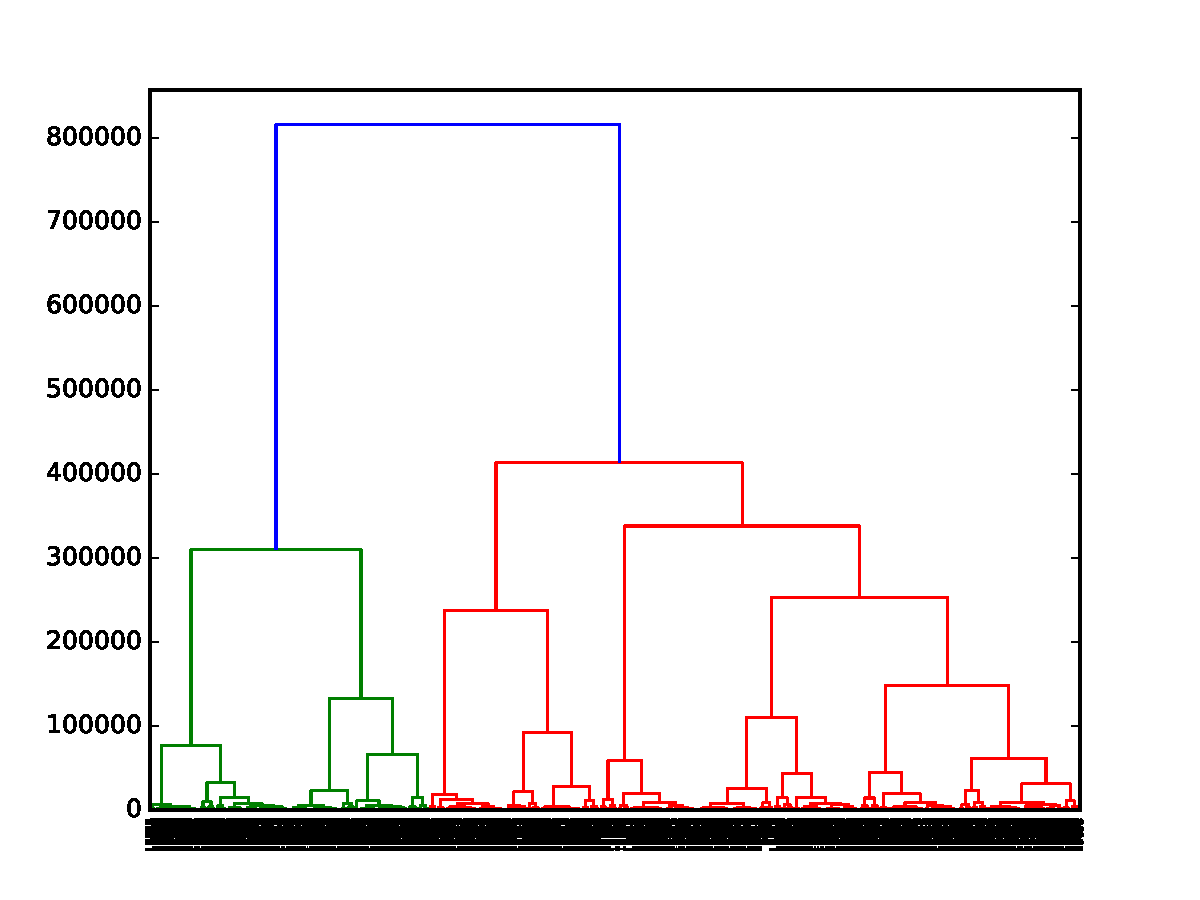
\includegraphics[scale=0.6]{dendrogram.pdf}
    \caption{Dendrogram of training data}
    \label{fig:dendrogram}
\end{figure}

\subsection{Simplifying labels}
Another step that was considered during experiments was the aggregation of habitat labels. The original training data contained 24 separate labels determined through an automated clustering procedure using Dirichlet Processes. Because of the uneven distribution of these labels(\todo{generate these images} \ref{fig:singlelabeldistr} and \ref{fig:multilabeldistr}), with the occurrence of some too insignificant for any machine learning algorithms to pick up, they were simplified in collaboration with ecological experts, who manually identified which of the 24 labels were in fact of the same class - for example, 5 separate classes of coral may have been indistinguishable to the average person, and were hence grouped into a single label. This allowed the near-non-occurring labels to be grouped together with more commonly occurring ones, whilst also allowing a different level of granularity in training models/forming predictions that could be used if only a rough approximation of an area's benthic map were required.

\begin{figure}[H]
    \begin{minipage}{.49\linewidth}
        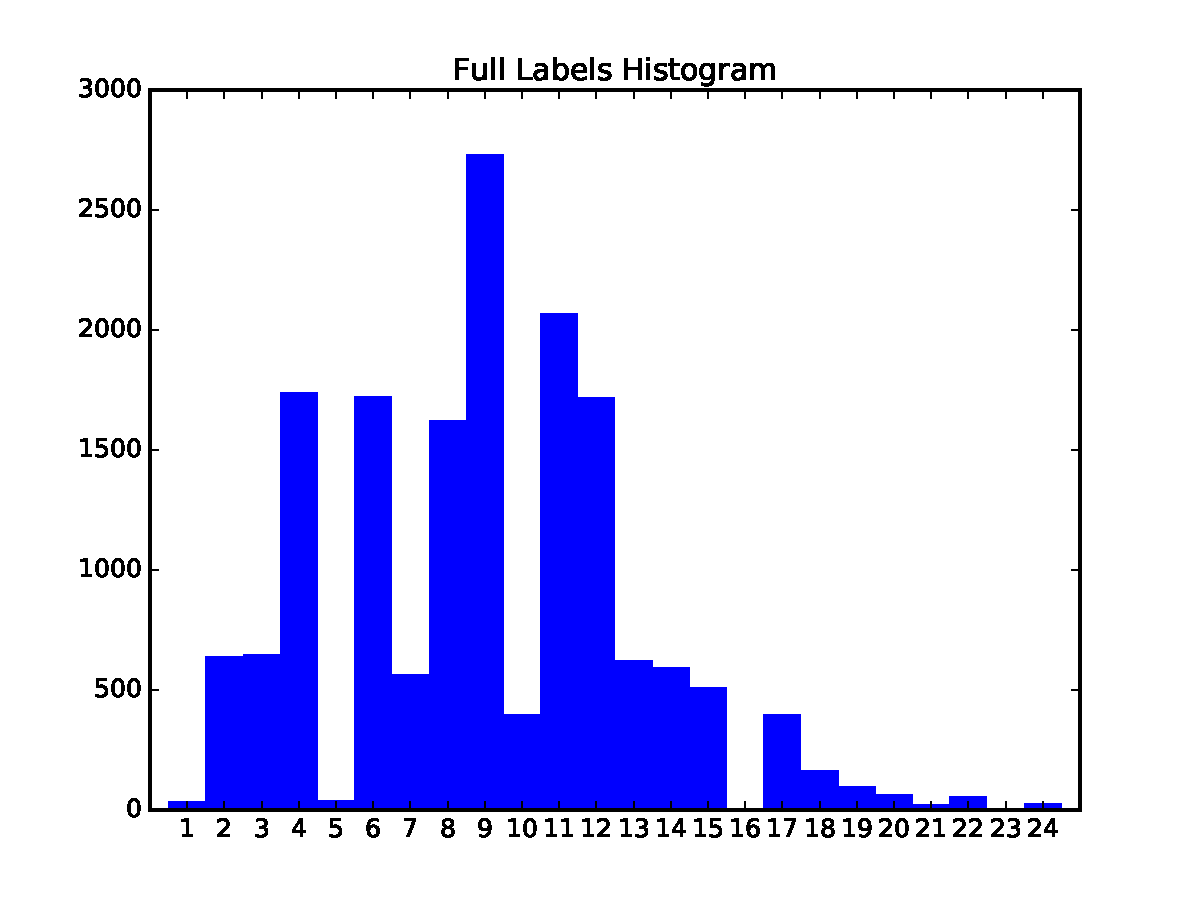
\includegraphics[width=\linewidth]{hist_full_labels.pdf}
        \caption{Distribution of labels in original dataset}
        \label{fig:singlelabeldistr}
    \end{minipage}
    \hfill
    \begin{minipage}{.49\linewidth}
        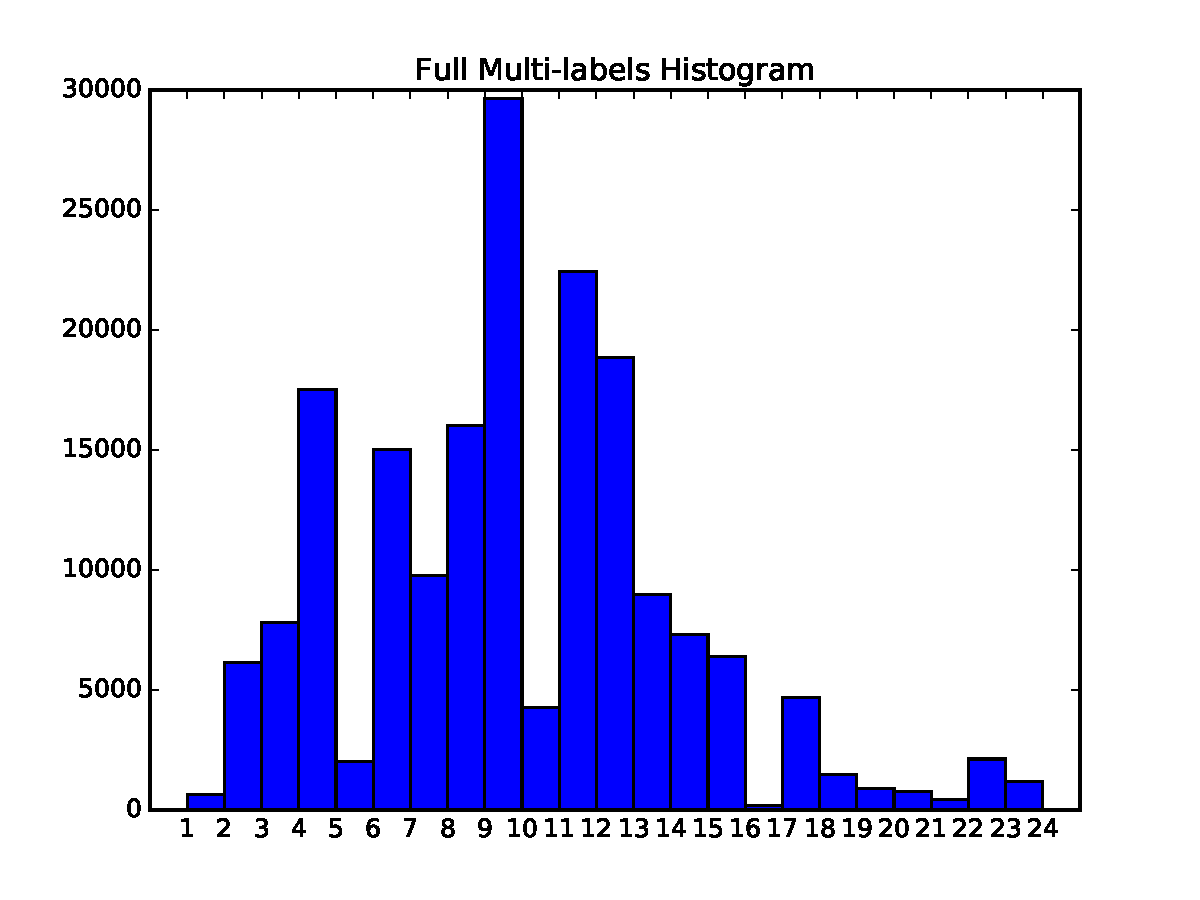
\includegraphics[width=\linewidth]{hist_full_multi_labels.pdf}
        \caption{Distribution of labels in multi-label outputs}
        \label{fig:multilabeldistr}
    \end{minipage}
\end{figure}

\section{Illustrative Example}

The differences between a Gaussian Process which provides the probability distribution of possible labels compared to the Dirichlet Multinomial Regressor which provides the distribution of actual labels at a point, are highlighted in the illustrative example below. \todo{generate toy example with a mixed label A,B region and separate regions of just A, just B}

From this basic example, it is apparent that in the area where there is an even mix of labels A, B, the Gaussian Process' predictions are both noisy and uncertain about their predictions, where human intervention would be required to observe the fact that it is in fact a consistent mix of both. In contrast, the dirichlet multinomial regressor is more confident in the fact that that area does in fact have a mix of labels. 

\chapter{Evaluation and Discussion} \label{chap:evaluation}

This chapter will assess some of the problems with the results from the experiments in \Cref{chap:experiments}, the implications they may have, and possible courses of action to resolve such issues. Limitations in general with different aspects of the study are also highlighted as appropriate.

\section{Data Limitations}

\textbf{Spread of habitat labels} - There were a number of properties regarding the data collected that likely had a negative effect on the experimental results, detracting from the figures surrounding accuracy scores, but not from the broader observations about qualitative use of predictions themselves. There is a significant class imbalance in the training data (\Cref{fig:multilabeldistr}), with each of the labels $1, 16, 18-21, 23, 24$ in particular having a total count of less than $10\%$ of the average label counts. Whilst habitat mapping is not inherently a class-imbalance problem, the models explored do not account for this, becoming most notable when assessing f-scores, even when considering the simplified labels.

\begin{table}[H]
    \caption{F-scores over labels}
\end{table}

\textbf{Image Clusters} - For any unsupervised algorithm that clusters images based on any number of properties from the image alone, any necessary pre-processing or normalisation of them needs to be done beforehand, to prevent unintended features such as discrepancies in lighting or saturation from misleading the clustering process. This was not the case here, however, as the lighting was at times quite variable at least in between clusters, and in one particular case, resulted in pitch-black photos. It appears that photos were taken during both the day and night, causing at least part of the difference, a problem that can be resolve with relative ease by restricting data collection to either day or night time. Of course, interferences can come from external sources independent of the time of day, so it would be ideal to pre-process all images to begin with. 

\subsection{Limitations}

\begin{itemize}
    \item data simply not varied enough/uninteresting habitat spread in Scott Reef?
    \item training data doesn't explore any particular area exhaustively - hard to verify how accurate any model is even if cross validation scores are high
    \item from the full 24 clusters, it's apparent that some were clustered as a result of lighting, unfortunately not a desired behaviour ==> possible future work is to first 'normalize' the contrast/visual properties of the images beforehand \todo{(Get a citation for this, I think it was an ACFR paper)}
    \item as a result of non-normalised images and hence somewhat flawed classifications, label 0 fails to be predicted often across most models tested, exacerbated in the 24-label case
        \begin{itemize}
            \item suggests that data may be insufficient, or that certain data from images may need to be incorporated into training data
        \end{itemize}
\end{itemize}

\chapter{Conclusion} \label{chap:conclusion}

Benthic habitat mapping is a relatively old concept, dating back at at least several decades when photos and videos became a viable method of capturing information about the benthos ~\citep{gibson07} as an alternative to earlier destructive methods of sediment sampling. However, the different sources of data required and the machine learning techniques needed to model the data to be able to predict properties about the benthos did not become more readily available until relatively recently. With tools such as multibeam echosounders for collecting acoustic backscatter data at scale, as well as extensive visual imaging of the benthos via autonomous underwater vehicles, it has become possible to collect large amounts of data about Earth's ocean to work with to gain a deeper understanding. Many studies to date have used machine learning algorithms such as SVMs and random forests on different types of data in different habitats and shown moderately good results, while more state of the art methods employ probabilistic methods such as Gaussian processes~\citep{bender12} that capture a richer set of information in the form of both predictions over possible labels as well as certainties around these predictions, or Gaussian mixture models~\citep{ahsan11} that are able to identify clusters that are individually multivariate Gaussians.

In this study, application of products of experts models was applied to Gaussian processes to lift the usual limitation on data sizes of several thousand points due to the time that would be needed to fit them. In fact, due to the requirement of multiple Gaussians processes to form GP classifiers, this several thousand is effectively scaled down by a factor proportional to the number of classes in the data. Experiments showed that for aggregated labels, the ensembles of experts were comparable in performance to the full GP, though the performance gap grew when dealing with the 24-label case, but keeping in mind that the GP became unusable on the full query data for predictions due to the time required. The predictions on the simple labels of the approximations also matched that of random forests and the distributions of the Diriclet multinomial's predictions.

As all the studies performed in the area of benthic habitat mapping deal with single-label outputs, they would be unable to account for and fully utilise multi-label count data, and resort to approximations by taking the most frequently occuring label per output. To assess the viability of working with multi-output data in benthic habitat mapping, the Dirichlet multinomial was used, serving exactly this purpose. 

\section{Future Work}

\begin{itemize}
    \item perform similar experiments on incrementally changing data every few years - observe biodiversity/habitat changes
    \item replace the simple activation function in the dirichlet multinomial with a more complex model like a GP
    \item previous work has been done for finding least certain areas of a GP to decide where to send AUV's to maximise resulting confidence in habitat labels - use entropy to be able to do the same with dirichlet multinomials, whilst overcoming the problem of areas with consistent heterogenous labels that otherwise confuse GPs
    \item combine habitat data with actual fauna distributions as well
    \item explore other multinomial prior distributions other than Dirichlet, such as Logit-normal distributions?
\end{itemize}

There a number of areas that would be pertinent to explore as an extension of this study, to further the usefulness of the data provided in terms of both the complexities of the underlying models used to predict data, as well as the contexts in which they are used.





%%%%%%%%%%%%
% End

% Bibliography
\bibliographystyle{style/mybibstyle}
{
\setstretch{1.25}
\cleardoublepage
\phantomsection
\bibliography{references}
}

%%%% Appendices
\appendix
addtocontents{toc}{\protect\setcounter{tocdepth}{1}}
% \chapter{Appendix}
things

\chapter{Appendix}
things

% input{wikifeats/wikifeats.tex}
% input{candcner/candcner.tex}
% input{comparedata/comparedata.tex}

\end{document}
